%==============================================================
% CV One-Pager Mejorado - Sebastián Mesch Henriques
%==============================================================
\documentclass[11pt,a4paper]{article}

\usepackage[utf8]{inputenc}
\usepackage[T1]{fontenc}
\usepackage[spanish]{babel}
\usepackage{lmodern}
\usepackage[margin=0.75cm,top=0.5cm,bottom=0.6cm]{geometry}
\usepackage{xcolor}
\usepackage{hyperref}
\usepackage{graphicx}
\usepackage{tikz}
\usetikzlibrary{calc}
\usepackage{calc}

%-------------------- Colores --------------------
\definecolor{primary}{HTML}{1F3A5F}
\definecolor{accent}{HTML}{2E86AB}

\pagestyle{empty}
\setlength{\parindent}{0pt}
\setlength{\parskip}{4pt}

%-------------------- Comandos personalizados --------------------
\newcommand{\cvtitle}[1]{ %
  {\color{primary}\bfseries\large\uppercase{ #1 }}
  {\color{accent}\hrule height 0.5pt}\vspace{6pt}
}

\newcommand{\cvexperience}[4]{ %
  {\bfseries\normalsize\color{primary} #1 } \hfill {\small\color{gray} #3 }\\
  {\small\color{accent}\itshape #2 } \\
  {\small #4 }\par
  \vspace{5pt}
}

\newcommand{\cveducation}[3]{ %
  {\bfseries\small\color{primary} #1 } \hfill {\small\color{gray} #3 }\\
  {\small #2 }\par
}

%-------------------- ATS Friendly Unicode --------------------
\input{glyphtounicode}
\pdfgentounicode=1

%==============================================================
\begin{document}

% ==================== IMAGEN DE PERFIL REDONDEADA ====================
\begin{tikzpicture}[remember picture, overlay]
  \node[anchor=north east, inner sep=0cm] at ($ (current page.north east) + (-0.75cm, -0.5cm) $) { %
    \begin{tikzpicture}
      \clip (0,0) circle (1.5cm);
      \node[anchor=center] at (0,0) {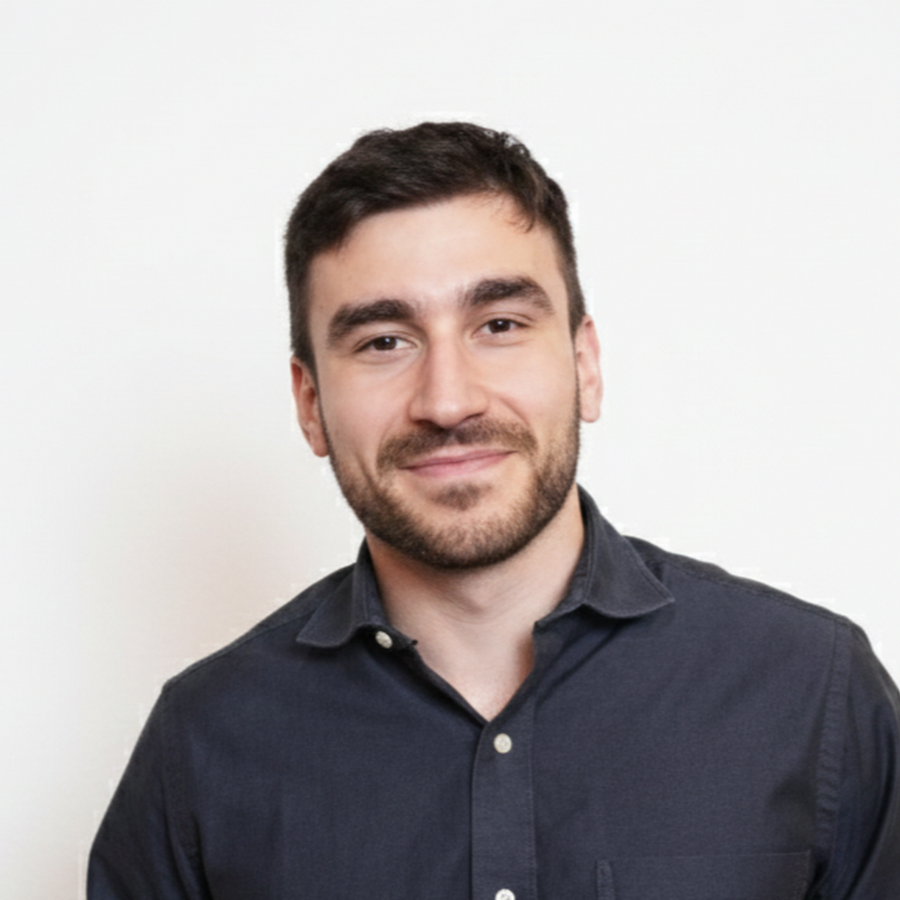
\includegraphics[width=3cm, height=3cm]{../assets/perfil.png}};
    \end{tikzpicture}
  };
\end{tikzpicture}

% ==================== ENCABEZADO ====================
\begin{minipage}[t]{0.65\textwidth}
{\bfseries\LARGE \uppercase{Sebastián Mesch Henriques}}\\[1pt]
{\color{accent}\large AI Engineer Jr. | Data Scientist | Neurocientífico }\\[3pt]
\end{minipage}

% ==================== CONTACTO ====================
{\normalsize
\href{mailto:lic.mesch@gmail.com}{lic.mesch@gmail.com} $|$
(+54 9) 11 3757 2384 $|$
CABA, Argentina\\
\href{ https://github.com/SMESCH1 }{GitHub} $|$
\href{ https://smesch1.github.io/ }{Portfolio} $|$
\href{ https://linkedin.com/in/sebastian-mesch-henriques }{LinkedIn}
}

{\color{accent}\hrule height 0.5pt}\vspace{16pt}

% ==================== PERFIL ====================
\cvtitle{ Perfil }
{\normalsize Ingeniero en IA con background en Neurociencias. Especialista en arquitecturas con LLMs, ML/DL y automatización de datos. Experiencia en liderazgo técnico, educación y research científico. }
\vspace{8pt}

% ==================== EXPERIENCIA ====================
\cvtitle{ Experiencia }


\cvexperience{Científico de Datos}{Universidad Favaloro}{2026 - Act.}{Análisis de datos para Orientación Vocacional. *(Stack: Python, Pandas, Power BI)*}

\cvexperience{Mentor en IA}{Humai}{2026 - Act.}{Guía técnica en IA y Neurociencias, enfocado en proyectos aplicados de ML/DL.}

\cvexperience{Coordinador Académico}{Humai}{2022 - 2026}{Liderazgo de equipo y automatización de pipelines de datos, reduciendo tiempos de reporte. *(Stack: Python, SQL)*}

\cvexperience{Quality Control Manager}{Further Languages}{2020 - 2022}{Gestión B2B, dashboards de KPIs y automatización de datos.}

\cvexperience{Investigador Asociado}{Universidad Favaloro}{2019 - 2023}{Desarrollo de modelos ML para neuroimagen y co-autoría de publicaciones. *(Stack: Scikit-learn, fMRI)*}

\cvexperience{Investigador}{BID}{2019 - 2020}{Investigación y análisis de datos sobre vivienda e informalidad.}



% ==================== EDUCACIÓN & CERTIFICACIONES ====================
\begin{minipage}[t]{0.48\textwidth}
\cvtitle{ Educación }

\cveducation{Maestría en IA}{UDESA}{2025 - Act.}

\cveducation{Lic. Psicología}{Univ. Favaloro}{2018 - 2024}

\cveducation{Data Scientist}{Coder House}{2022 - 2023}

\cveducation{Secundarios}{Colegio Nac. Bs As}{2012 - 2016}

\end{minipage}
\hfill
\begin{minipage}[t]{0.48\textwidth}
\cvtitle{ Certificaciones }
{\normalsize

Certified AI Practitioner (AWS 2025) \\

LLMs \& Deep Learning (Humai 2025) \\

Data Science (Coder House 2023) \\

Big Data (Codo a Codo 2022) \\

}
\end{minipage}

\vspace{8pt}

% ==================== HABILIDADES ====================
\cvtitle{ Habilidades }
{\normalsize

Data & ML: Python, SQL, Scikit-learn, Pandas, NumPy, TensorFlow \\

Dev & Ops: Git, GitHub, Docker, Airflow, dbt, HTML/CSS \\

IA: LLMs, AI Agents, Claude Code, RAG \\

Blandas: Liderazgo técnico, Comunicación interdisciplinaria, Pensamiento Crítico, Resolución de Problemas \\

}

\vspace{8pt}

% ==================== IDIOMAS & PUBLICACIONES ====================
\begin{minipage}[t]{0.48\textwidth}
\cvtitle{ Idiomas }
{\normalsize

Español -- Nativo \\

Inglés -- C2 (CPE Cambridge) \\

Francés -- Básico \\

}
\end{minipage}
\hfill
\begin{minipage}[t]{0.48\textwidth}
\cvtitle{ Publicaciones }
{\small

Psicología y Sociedad (Scielo Brasil 2025) \\

Revisión Sistemática (Univ. Favaloro 2025) \\

Soc. Argentina de Neurociencias (2024) \\

}
\end{minipage}

\end{document}